
\chapter{MISP}
\newpage

\section{lecture}

\subsection{Traffic Light Protocol (TLP)}

\begin{description}
   \item[\textcolor{red}{TLP:RED}] = Not for disclosure, restricted to participants only.
   \begin{itemize}
       \item Sources may use TLP:RED when information cannot be effectively acted upon by additional parties, and could lead to impacts on a party's privacy, reputation, or operations if misused.
       \item Recipients may not share TLP:RED information with any parties outside of the specific exchange, meeting, or conversation in which it was originally disclosed.
       \item In the context of a meeting, TLP:RED information is limited to those present at the meeting.
       \item In most circumstances, TLP:RED should be exchanged verbally or in person.
   \end{itemize}

   \item[\textcolor{orange}{TLP:AMBER}] = Limited disclosure, restricted to participants' organizations.
   \begin{itemize}
       \item Sources may use TLP:AMBER when information requires support to be effectively acted upon, yet carries risks to privacy, reputation, or operations if shared outside of the organizations involved.
       \item Recipients may only share TLP:AMBER information with members of their own organization, and with clients or customers who need to know the information to protect themselves or prevent further harm.
       \item Sources are at liberty to specify additional intended limits of the sharing: these must be adhered to.
   \end{itemize}

   \item[\textcolor{green}{TLP:GREEN}] = Limited disclosure, restricted to the community.
   \begin{itemize}
       \item Sources may use TLP:GREEN when information is useful for the awareness of all participating organizations as well as with peers within the broader community or sector.
       \item Recipients may share TLP:GREEN information with peers and partner organizations within their sector or community, but not via publicly accessible channels.
       \item Information in this category can be circulated widely within a particular community.
       \item TLP:GREEN information may not be released outside of the community.
   \end{itemize}

   \item[TLP:WHITE] = Disclosure is not limited.
   \begin{itemize}
       \item Sources may use TLP:WHITE when information carries minimal or no foreseeable risk of misuse, in accordance with applicable rules and procedures for public release.
       \item Subject to standard copyright rules, TLP:WHITE information may be distributed without restriction.
   \end{itemize}
\end{description}

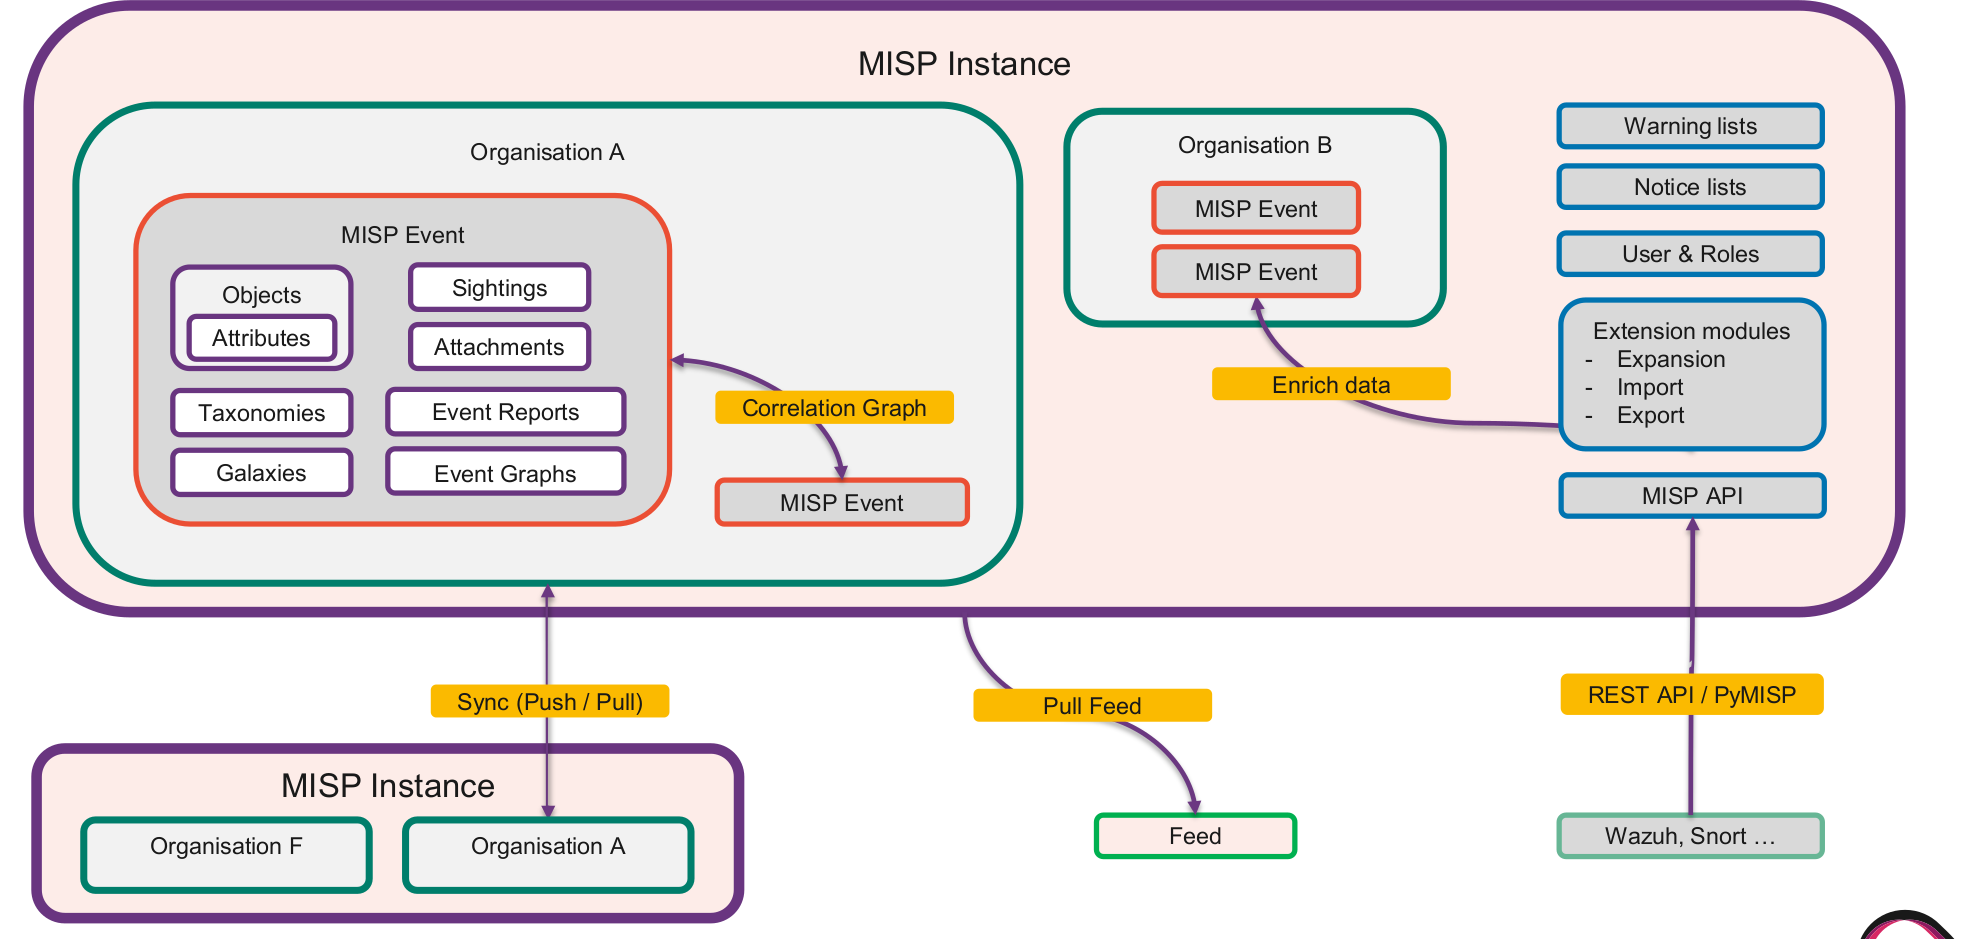
\includegraphics[width=\textwidth]{resources/10-misp-overview.png}
\section{MISP: Malware Information Sharing Platform}

\subsection{Introduction}

\subsubsection{What is MISP}
MISP is an open-source threat intelligence platform designed to facilitate the sharing and exchange of:
\begin{itemize}
    \item Threat intelligence data
    \item Indicators of Compromise (IoCs)
    \item Information about targeted malware and attacks
    \item Financial fraud intelligence
    \item Any intelligence within trusted communities
\end{itemize}

\subsubsection{Why Threat Intelligence Sharing Matters}
\begin{itemize}
    \item Cybersecurity is fundamentally a team sport
    \item Adversaries actively share information, expertise, and code
    \item Without collaboration, defensive teams fall behind
    \item Over 6000 organizations worldwide use MISP
    \item Creates a network effect in threat detection and response
\end{itemize}

\subsubsection{Intelligence Sources}
\paragraph{Open Source Intelligence (OSINT)}
\begin{itemize}
    \item Twitter with keywords/hashtags (Tweetdeck)
    \item MalwareBazaar
    \item URLhaus
    \item GitHub resources
    \item Public threat feeds
\end{itemize}

\paragraph{Closed Source Intelligence (CSINT)}
\begin{itemize}
    \item Microsoft Exchange data
    \item Email intelligence
    \item PDF analysis
    \item Private threat feeds
    \item Internal telemetry
\end{itemize}

\subsubsection{Sightings}
MISP Sightings provide important contextual information:
\begin{itemize}
    \item Indicates when attributes are seen in the wild
    \item Can mark false positives
    \item Provides expiration dates for attributes
    \item Types of sightings:
        \begin{itemize}
            \item Positive sighting (confirmation)
            \item False positive (incorrect detection)
            \item Expiration (no longer valid)
        \end{itemize}
    \item Helps maintain data quality
    \item Supports threat intelligence lifecycle
\end{itemize}

\subsubsection{Proposals}
Collaborative feature for event modification:
\begin{itemize}
    \item Allows users to propose changes to events
    \item Use cases:
        \begin{itemize}
            \item Correct typos in attributes
            \item Add missing information
            \item Update outdated data
            \item Enhance existing attributes
        \end{itemize}
    \item Workflow:
        \begin{itemize}
            \item User submits proposal
            \item Event owner gets notified
            \item Owner can approve or discard the proposal
            \item Changes are tracked for accountability
        \end{itemize}
    \item Maintains data integrity while enabling collaboration
    \item Supports community-driven intelligence improvement
\end{itemize}

\subsubsection{Event Reports}
Documentation capability within events:
\begin{itemize}
    \item Can be manually written for additional context
    \item Automatically compiled from attributes/objects
    \item Supports Markdown format
    \item CRUD operations available
    \item Helps provide narrative context to technical data
    \item Useful for:
        \begin{itemize}
            \item Incident documentation
            \item Analysis summaries
            \item Investigation notes
            \item Context sharing
        \end{itemize}
\end{itemize}

\paragraph{Event Properties}
\begin{description}
    \item[Date] When the event occurred
    \item[Distribution] Sharing scope of the event
    \item[Threat Level] High, Medium, Low, Undefined
    \item[Analysis] Initial, Ongoing, Complete
    \item[Event Info] Title/description
    \item[Extends Event] Related event reference
\end{description}

\subsubsection{Attributes}
Event descriptors that can include:
\begin{itemize}
    \item Network indicators (IP addresses, domains)
    \item System indicators (memory strings, file hashes)
    \item Financial indicators (bank accounts, transaction IDs)
    \item Personal information (when relevant)
\end{itemize}

\subsubsection{Objects}
Grouped attributes that belong together:
\begin{itemize}
    \item Person object (name, address, phone, etc.)
    \item Email object (subject, sender, attachments)
    \item File object (name, size, hashes)
    \item Network connection object
\end{itemize}

\subsubsection{Attachments}
Supports various attachment types:
\begin{itemize}
    \item Antivirus detection results
    \item Payload samples
    \item Network captures (PCAP)
    \item External analysis reports
    \item Support documentation
\end{itemize}

\subsubsection{Event Visualization}
\begin{itemize}
    \item Event Graphs for visual representation
    \item Shows relationships between elements
    \item Makes complex events easier to understand
    \item Supports investigation workflows
\end{itemize}

\subsubsection{Taxonomies}
Classification system with:
\begin{itemize}
    \item 127+ predefined taxonomy libraries
    \item Custom taxonomy support
    \item Namespace:predicate=value format
    \item Examples include TLP, MITRE ATT\&CK
\end{itemize}

\subsubsection{Galaxies}
Complex object expression system:
\begin{itemize}
    \item Used for larger contextual objects
    \item Contains clusters of related elements
    \item Examples include MITRE ATT\&CK matrices
    \item Supports threat actor tracking
\end{itemize}

\subsection{Evaluation}

\subsubsection{Correlation}
Automatic relationship detection:
\begin{itemize}
    \item Between events and attributes
    \item Based on common indicators
    \item Supports investigation
    \item Visual correlation graphs
\end{itemize}

\subsubsection{Warning Lists}
\begin{itemize}
    \item Lists of known false positives
    \item Common error patterns
    \item Helps reduce false alerts
    \item Continuously updated
\end{itemize}

\subsubsection{Notice Lists}
Inform users about:
\begin{itemize}
    \item Legal implications
    \item Privacy concerns
    \item Policy requirements
    \item Technical considerations
    \item GDPR compliance
\end{itemize}

\subsection{Sharing}

\subsubsection{Distribution Models}
Five levels of sharing:
\begin{itemize}
    \item Your organization only
    \item This community only
    \item Connected communities
    \item All communities
    \item Sharing groups
\end{itemize}

\subsubsection{Synchronization}
\begin{itemize}
    \item Push mode: Real-time sharing
    \item Pull mode: On-demand updates
    \item Configurable sharing rules
    \item Tag-based filtering
\end{itemize}

\subsubsection{Feeds}
\begin{itemize}
    \item Remote and local feed support
    \item Multiple format support
    \item Regular update intervals
    \item Redis caching for correlation
\end{itemize}

\subsection{Miscellaneous}

\subsubsection{API Capabilities}
\begin{itemize}
    \item REST API
    \item PyMISP Python library
    \item Authentication via API keys
    \item Comprehensive documentation
\end{itemize}

\subsubsection{Expansion Modules}
Types of modules:
\begin{itemize}
    \item Expansion (enrichment)
    \item Export (format conversion)
    \item Import (data ingestion)
    \item Integration modules
\end{itemize}

\subsection{Outlook}
Future developments and applications:
\begin{itemize}
    \item Growing community adoption
    \item Enhanced automation capabilities
    \item Improved correlation features
    \item Extended integration options
    \item Advanced visualization tools
\end{itemize}


\section{exercise}
